% ======================= CHƯƠNG 3: PHƯƠNG PHÁP ==========================
\chapter{Phương pháp}

Chương này mô tả tập dữ liệu, ba kiến trúc, pipeline huấn luyện chung, các chỉ số đánh giá và bộ giải mã được đề xuất. Các siêu tham số được nêu rõ ràng để có thể tái lập các thí nghiệm.

\section{Tập dữ liệu: Cholec80}

Mọi thí nghiệm đều dùng tập dữ liệu công khai Cholec80: tám mươi video cắt túi mật nội soi, với một nhãn pha và các nhãn dụng cụ trên mỗi khung hình. Theo đúng quy ước thông dụng, các video được chia theo bệnh nhân thành 40 video huấn luyện (mã 1--40), 20 video kiểm định (mã 41--60), và 20 video kiểm tra (mã 61--80). Khung hình được lấy ở tốc độ một khung mỗi giây bằng OpenCV; các nhãn pha vốn ở 25~fps được lấy mẫu lại cho khớp. Mỗi khung hình được đổi kích thước về $224 \times 224$ điểm ảnh và chuẩn hóa theo trung bình và độ lệch chuẩn của ImageNet.

Trong lúc huấn luyện, cùng một bộ tăng cường dữ liệu nhẹ --- lật ngang ngẫu nhiên, xoay tới $10^\circ$, cắt ngẫu nhiên với biên 10\%, và rung màu (colour jitter) --- được áp dụng cho mọi khung hình trong một chuỗi để chuỗi giữ được tính nhất quán. Mỗi mẫu đầu vào là tám khung hình liên tiếp ở một khung mỗi giây, cho tám giây ngữ cảnh.

\begin{table}[H]
\centering
\caption{Phân bố các pha trong tập huấn luyện Cholec80 (1~fps).}
\label{tab:phase_distribution}
\begin{tabular}{clrr}
\toprule
\textbf{Mã} & \textbf{Pha} & \textbf{Số khung} & \textbf{Tỷ lệ} \\
\midrule
0 & Chuẩn bị                   & 3.758  & 4,4\% \\
1 & Bóc tách tam giác Calot    & 36.886 & 42,7\% \\
2 & Kẹp và cắt                 & 7.329  & 8,5\% \\
3 & Bóc tách túi mật           & 24.119 & 27,9\% \\
4 & Đóng gói túi mật           & 3.716  & 4,3\% \\
5 & Làm sạch và đông máu       & 7.222  & 8,4\% \\
6 & Lấy túi mật ra             & 3.314  & 3,8\% \\
\bottomrule
\end{tabular}
\end{table}

Pha phổ biến nhất (Bóc tách tam giác Calot) nhiều hơn pha hiếm nhất (Lấy túi mật ra) theo tỷ lệ 11,1 trên 1. Đây chính là sự mất cân bằng mà pipeline huấn luyện được xây dựng để xử lý. Hình~\ref{fig:vn_class_distribution} cho thấy phân bố trên cả ba tập.

\begin{figure}[H]
\centering
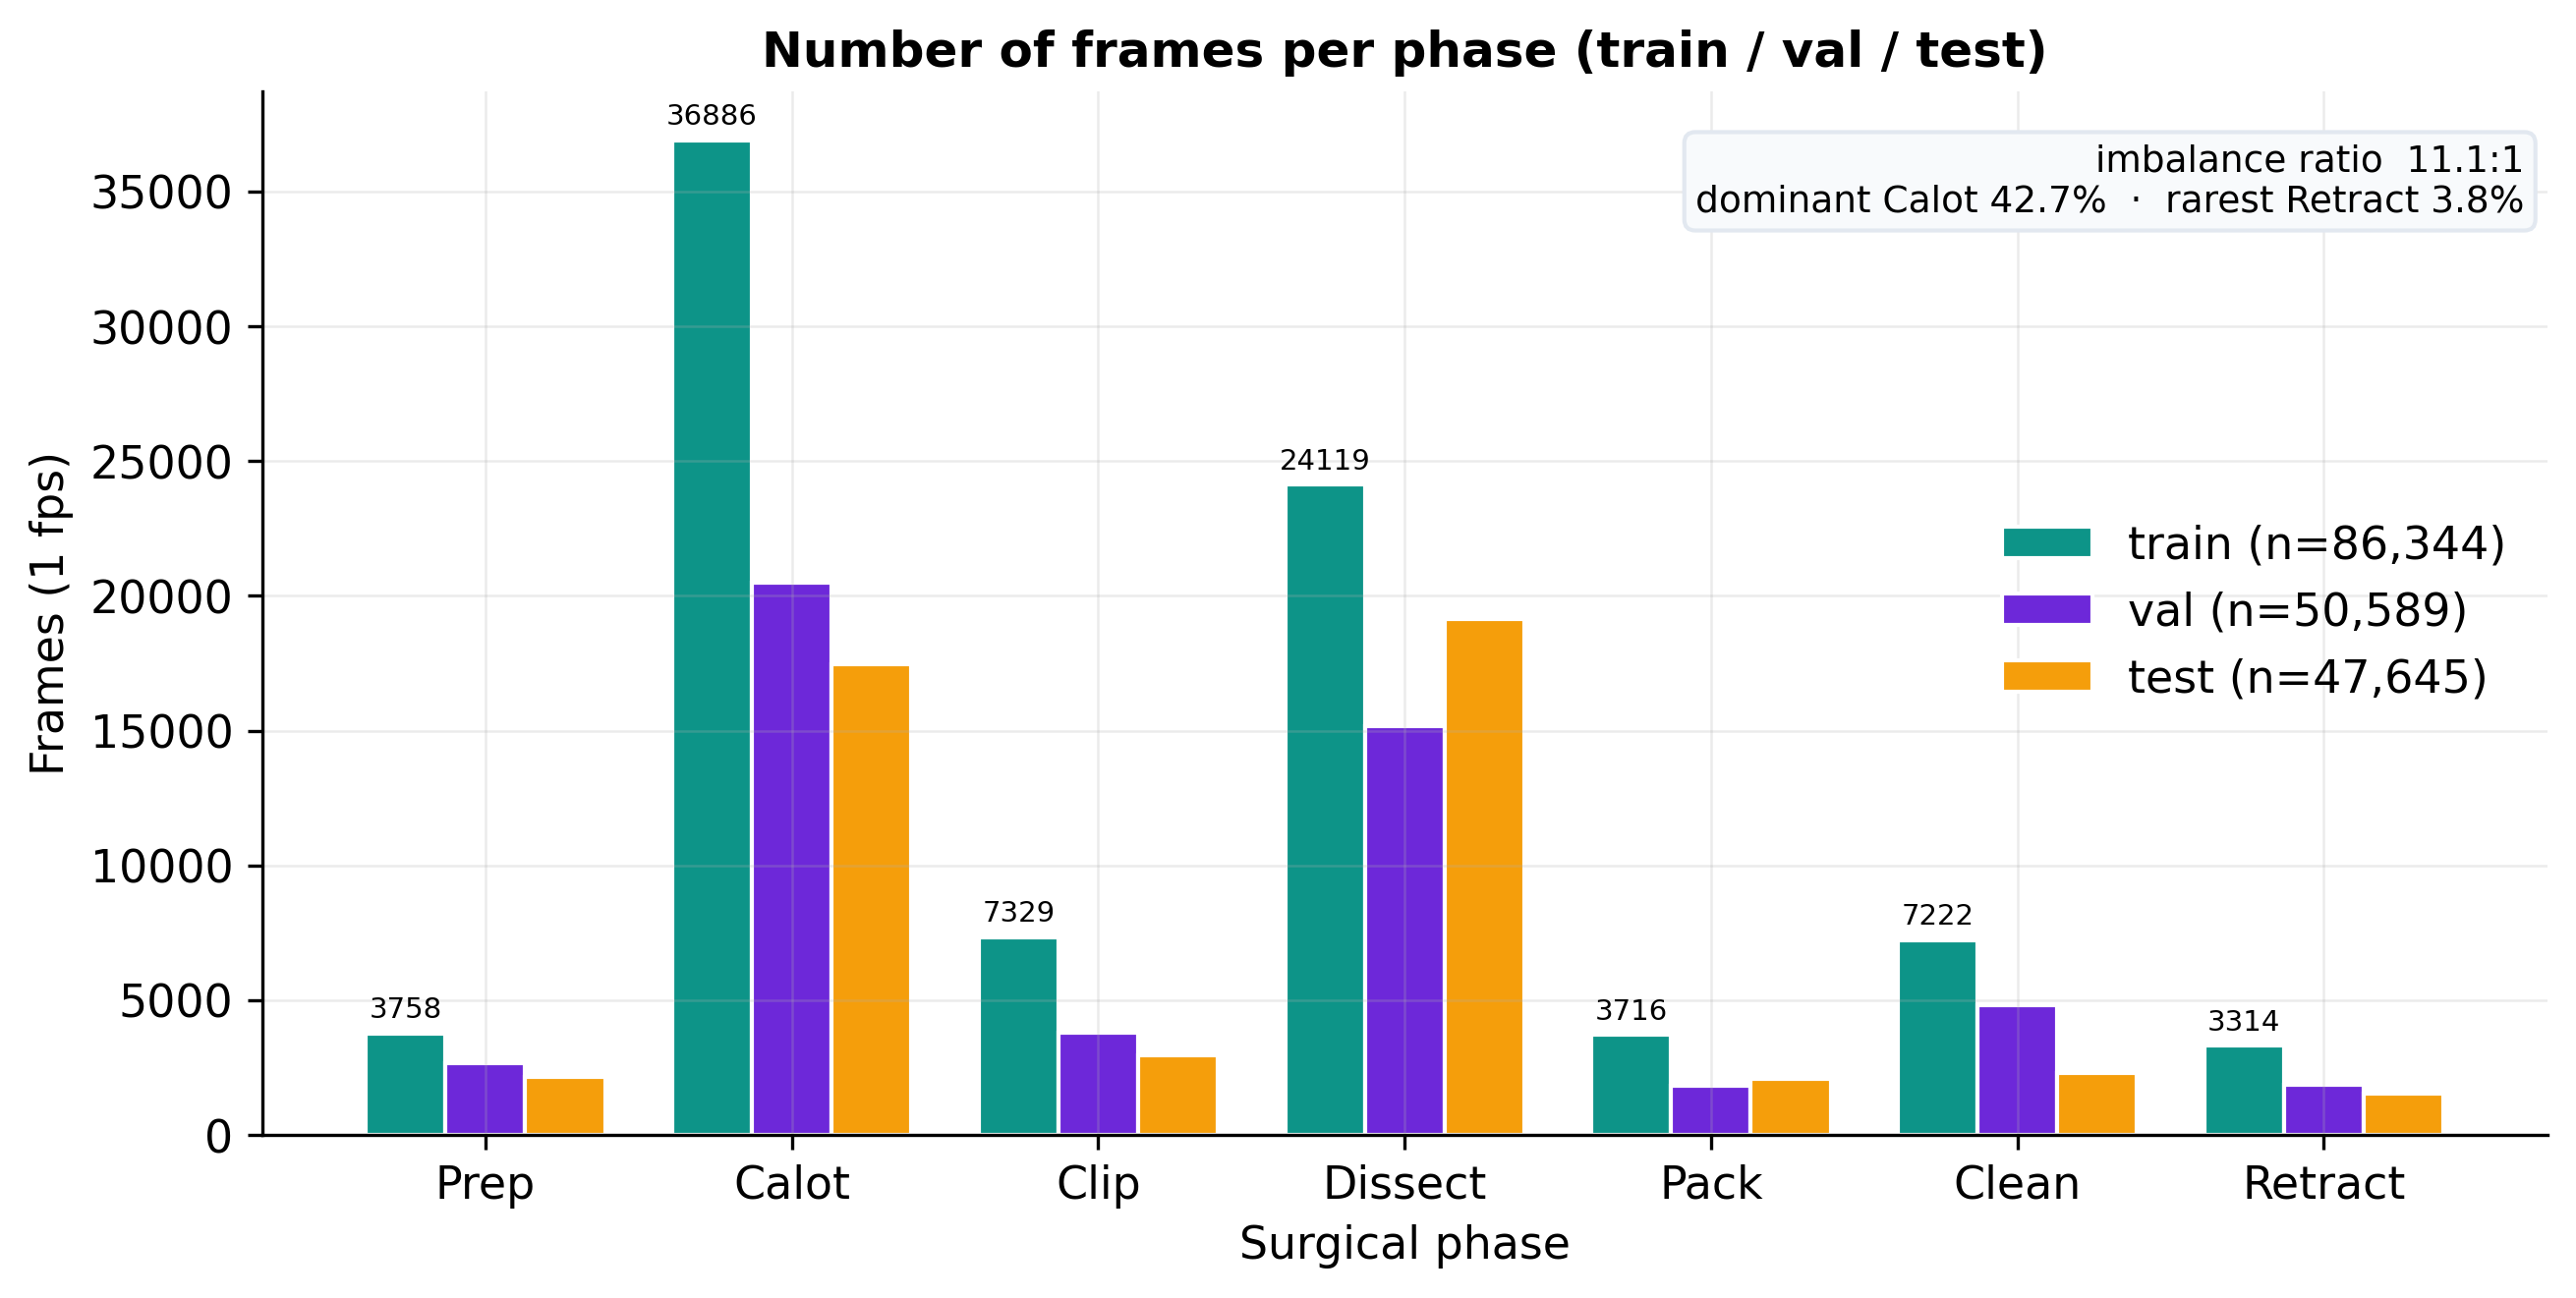
\includegraphics[width=\textwidth]{figures/class_distribution.png}
\caption{Số khung hình của mỗi pha trong các tập huấn luyện, kiểm định và kiểm tra. Các pha phổ biến (Calot, Bóc tách) chiếm ưu thế, còn các pha kết thúc (Đóng gói, Lấy ra) thì hiếm; tỷ lệ này tương tự nhau giữa các tập.}
\label{fig:vn_class_distribution}
\end{figure}

\section{Các Kiến trúc Mô hình}

Ba kiến trúc được so sánh, gọi là M1, M2 và M3. Cả ba có cùng cấu trúc tổng thể, minh họa trong Hình~\ref{fig:vn_transfer_learning}: một mạng nền biến mỗi trong tám khung hình thành một vec-tơ đặc trưng, một mô hình theo thời gian đọc chuỗi tám vec-tơ, và hai lớp đầu ra nhỏ dự đoán, cho từng khung hình, pha và những dụng cụ đang hiện diện. Tất cả mạng nền đều khởi tạo từ trọng số huấn luyện sẵn trên ImageNet, nạp qua thư viện \texttt{timm}.

\begin{figure}[H]
\centering
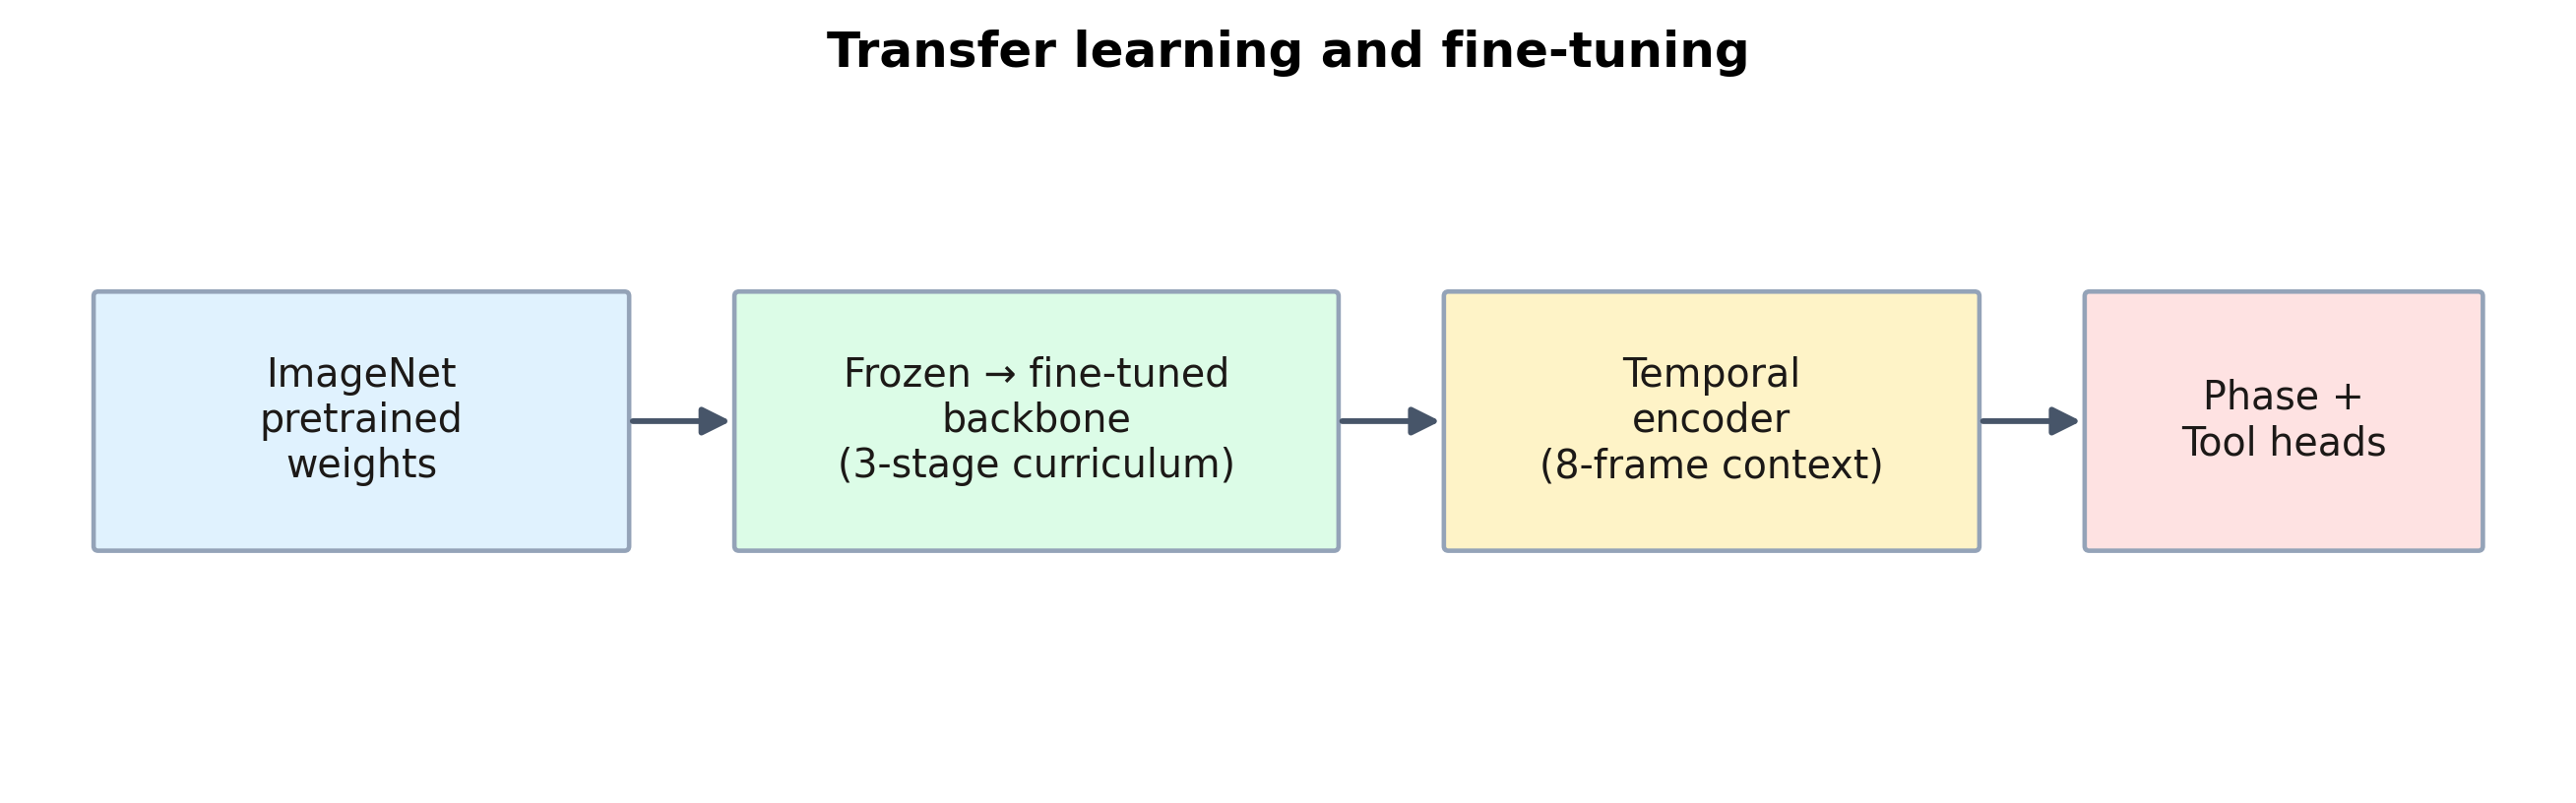
\includegraphics[width=\textwidth]{figures/transfer_learning.png}
\caption{Học chuyển giao (transfer learning) và tinh chỉnh. Mạng nền khởi đầu từ trọng số ImageNet và được tinh chỉnh qua ba giai đoạn; một mô hình theo thời gian gồm tám khung hình bổ sung ngữ cảnh; hai lớp đầu ra dự đoán pha và dụng cụ.}
\label{fig:vn_transfer_learning}
\end{figure}

\subsection{M1 --- ResNet-50 + LSTM hai chiều}

Mạng nền là ResNet-50 với trọng số ImageNet, cho các đặc trưng 2048 chiều. Mô hình theo thời gian là một LSTM hai chiều hai lớp với kích thước ẩn 512. Số tham số huấn luyện: 35,7~M. Cấu hình này theo SV-RCNet.

\subsection{M2 --- EfficientNet-B3 + Mạng tích chập theo thời gian}

Mạng nền là EfficientNet-B3 (đầu ra 1536 chiều). Mô hình theo thời gian là một mạng tích chập theo thời gian hai giai đoạn với tám lớp giãn nở mỗi giai đoạn và 64 bộ lọc, một phiên bản nhỏ hơn của TeCNO để vừa với giới hạn bộ nhớ. Số tham số huấn luyện: 11,2~M.

\subsection{M3 --- Swin-Tiny + Transformer}

Mạng nền là Swin Transformer-Tiny (đầu ra 768 chiều). Mô hình theo thời gian là một bộ mã hóa Transformer ba lớp với sáu đầu (head), kích thước mô hình 384 và kích thước lớp truyền thẳng 768 --- được giữ nhỏ một cách có chủ ý để vừa với giới hạn 4~GB. Số tham số huấn luyện: 31,6~M.

Ở cả ba mô hình, một lớp dropout 0,3 được đặt giữa mô hình theo thời gian và các lớp đầu ra. Lớp đầu ra pha là một lớp tuyến tính cho bảy điểm số; lớp đầu ra dụng cụ cho bảy giá trị sigmoid độc lập.

\begin{table}[H]
\centering
\caption{Tóm tắt ba kiến trúc được đánh giá.}
\label{tab:vn_architectures}
\begin{tabular}{lllrl}
\toprule
\textbf{Mô hình} & \textbf{Mạng nền} & \textbf{Mô hình thời gian} & \textbf{Tham số (M)} & \textbf{Họ} \\
\midrule
M1 & ResNet-50      & LSTM hai chiều       & 35,7 & CNN + RNN \\
M2 & EfficientNet-B3 & TCN nhiều giai đoạn  & 11,2 & CNN + TCN \\
M3 & Swin-Tiny      & Bộ mã hóa Transformer & 31,6 & ViT + Chú ý \\
\bottomrule
\end{tabular}
\end{table}

\section{Pipeline Huấn luyện}

Pipeline huấn luyện được thiết kế xoay quanh sự mất cân bằng 11:1. Nó xử lý vấn đề theo bốn cách --- đánh trọng số lớp, làm mượt nhãn, nhiệm vụ dụng cụ phụ, và một lịch trình theo giai đoạn --- và nghiên cứu loại bỏ (Mục~\ref{sec:vn_ablation}) đo lường mức đóng góp của từng cách. Hình~\ref{fig:vn_training_pipeline} cho cái nhìn tổng quan.

\begin{figure}[H]
\centering
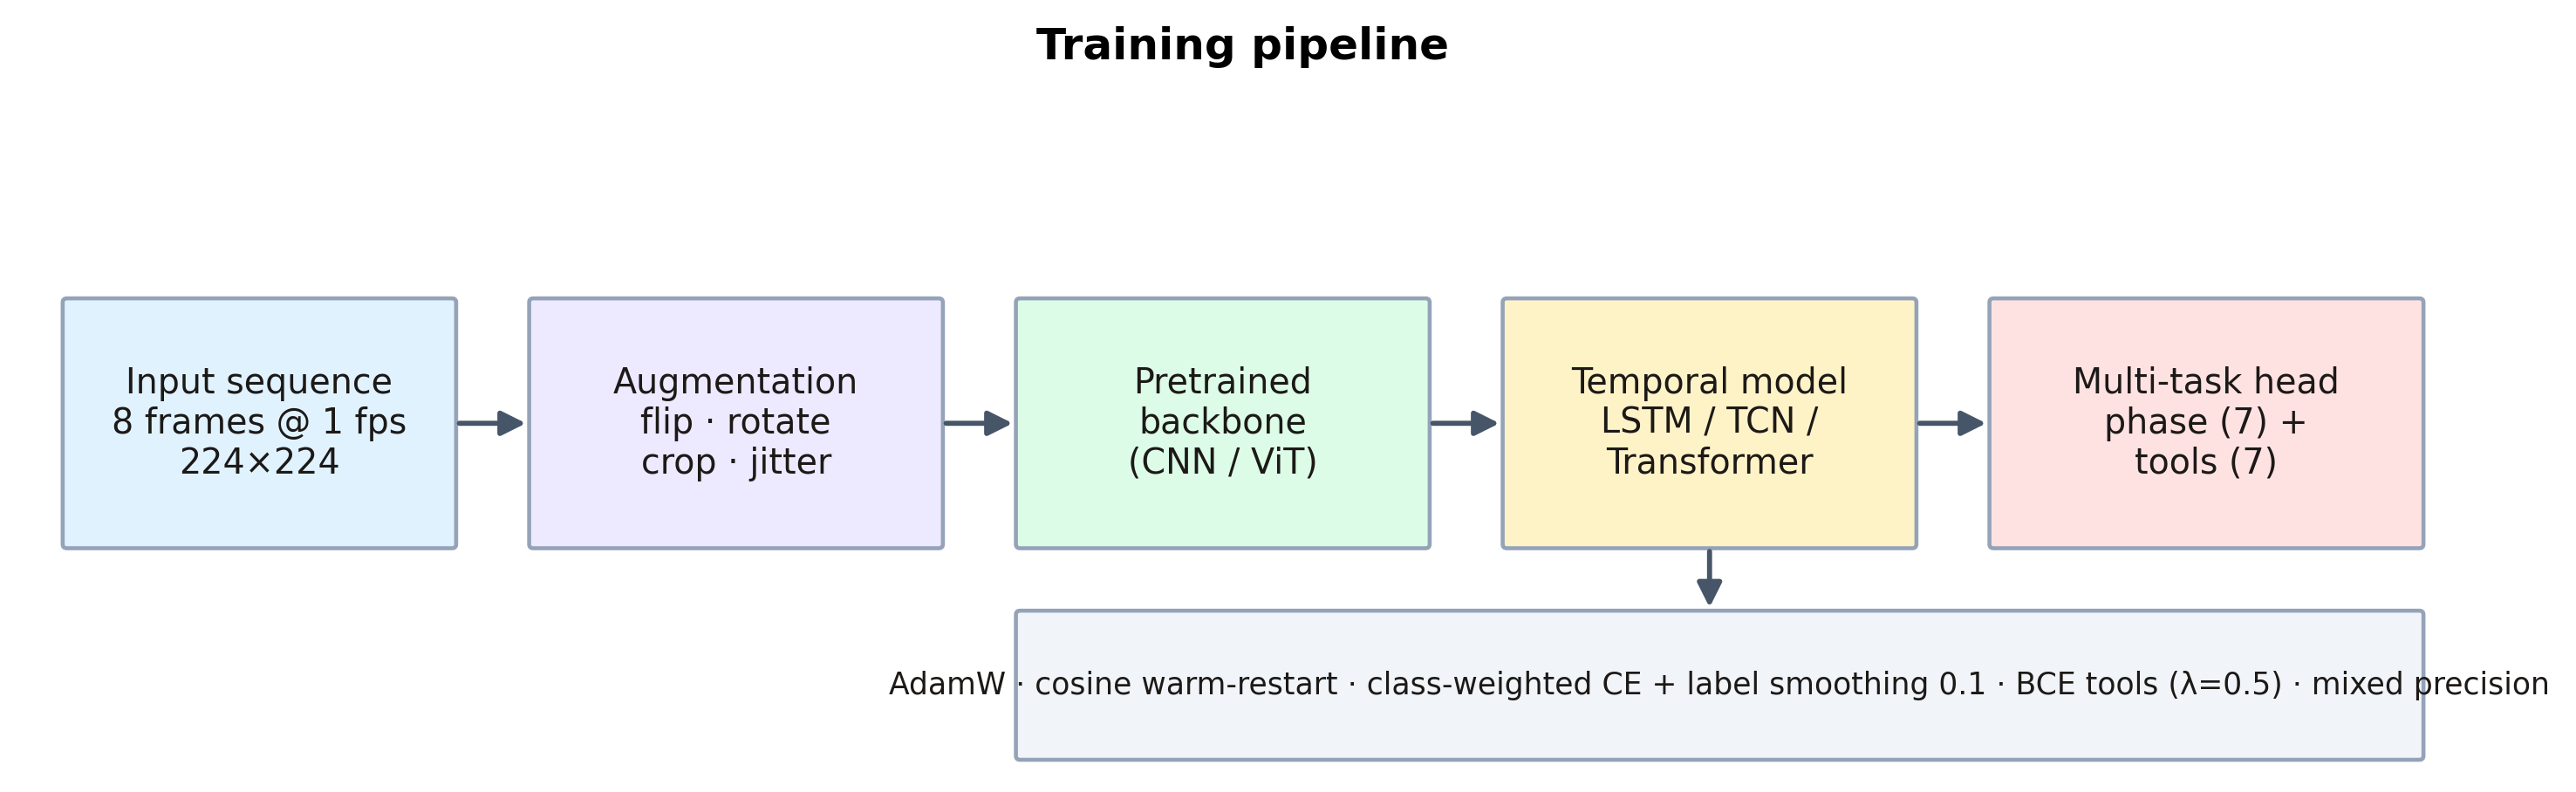
\includegraphics[width=\textwidth]{figures/training_pipeline.png}
\caption{Tổng quan pipeline huấn luyện. Một chuỗi tám khung hình được tăng cường, đi qua mạng nền và mô hình theo thời gian, rồi được phân loại bởi các lớp đầu ra. Huấn luyện dùng AdamW với lịch trình cosine, hàm cross-entropy có trọng số lớp kèm làm mượt nhãn cho pha, và cross-entropy nhị phân cho dụng cụ.}
\label{fig:vn_training_pipeline}
\end{figure}

\subsection{Hàm Mất mát}

Tổng mất mát là tổng có trọng số của một thành phần pha và một thành phần dụng cụ:
\begin{equation}
\mathcal{L} = \mathcal{L}_{\text{pha}}(z_{\text{pha}}, y_{\text{pha}}) + \lambda \cdot \mathcal{L}_{\text{dụng cụ}}(z_{\text{dụng cụ}}, y_{\text{dụng cụ}})
\label{eq:vn_total_loss}
\end{equation}
trong đó $\mathcal{L}_{\text{pha}}$ là cross-entropy có trọng số lớp kèm làm mượt nhãn 0,1, $\mathcal{L}_{\text{dụng cụ}}$ là cross-entropy nhị phân lấy trung bình trên bảy dụng cụ, và $\lambda = 0{,}5$. Trọng số lớp được tính tự động theo nghịch đảo tần suất lớp trên tập huấn luyện:
\begin{equation}
w_c = \frac{N}{C \cdot n_c}
\label{eq:vn_class_weight}
\end{equation}
trong đó $N$ là tổng số khung hình huấn luyện, $C = 7$ là số pha, và $n_c$ là số khung hình thuộc pha $c$. Các trọng số được co giãn để tổng bằng số lớp. Điều này bù lại mức mất cân bằng $11{,}1\times$ mà không bỏ qua các pha phổ biến.

\subsection{Lịch trình Ba Giai đoạn}

Huấn luyện chạy theo ba giai đoạn. Ở Giai đoạn 1 (5 epoch) mạng nền bị đóng băng và chỉ huấn luyện mô hình theo thời gian và các lớp đầu ra. Giai đoạn 2 (10 epoch) tiếp tục điều này. Ở Giai đoạn 3 (10 epoch) mạng nền được mở băng và toàn mạng được tinh chỉnh, với tốc độ học của mạng nền đặt nhỏ hơn phần còn lại mười lần. Các lần chạy loại bỏ dùng phiên bản ngắn hơn $3/6/6$.

\subsection{Tối ưu hóa}

Bộ tối ưu là AdamW với tốc độ học chính $1\times10^{-4}$, tốc độ học mạng nền $1\times10^{-5}$, suy giảm trọng số $1\times10^{-4}$, và một lịch trình cosine. Huấn luyện độ chính xác hỗn hợp (fp16) giữ bộ nhớ trong giới hạn 4~GB; gradient được cắt về chuẩn tối đa 1,0. Kích thước lô là 4 (M1), 8 (M2) và 4 (M3) --- mức lớn nhất vừa với bộ nhớ. Huấn luyện dừng sớm nếu Macro-F1 kiểm định không cải thiện trong năm epoch.

\subsection{Phần cứng và Phần mềm}

Mọi thí nghiệm chạy trên một GPU laptop NVIDIA GeForce RTX 2050 (4~GB) với CPU Intel Core i7 và 24~GB RAM, trên Windows 11, dùng Python 3.13, PyTorch 2.6 với CUDA 12.4, torchvision, timm, OpenCV và scikit-learn.

\section{Các Chỉ số Đánh giá}

Chỉ riêng độ chính xác là gây hiểu lầm trên Cholec80: một mô hình luôn dự đoán hai pha phổ biến sẽ có điểm cao trong khi bỏ qua các pha kết thúc ngắn. Vì vậy, các chỉ số sau được báo cáo kèm với độ chính xác.

\begin{itemize}
    \item \textbf{Macro-F1.} Trung bình của bảy điểm F1 theo từng pha, cho mọi pha trọng số như nhau bất kể nó phổ biến đến đâu. Đây là chỉ số chính để chọn mô hình.
    \item \textbf{Precision / Recall / F1 theo từng pha.} Trình bày kèm ma trận nhầm lẫn để thấy mỗi mô hình sai ở đâu.
    \item \textbf{Điểm Edit.} Một chỉ số ở mức đoạn, đánh giá chất lượng của \emph{chuỗi} pha dự đoán thay vì từng khung hình riêng lẻ.
    \item \textbf{Sai số hiệu chuẩn kỳ vọng (ECE) và Hàm log hợp lý âm (NLL).} Dùng trong phân tích hiệu chuẩn (Mục~\ref{sec:vn_calibration}).
\end{itemize}

Khi kiểm tra, pha dự đoán cho mỗi khung hình là pha có điểm cao nhất, và một bộ lọc trung vị độ dài mười lăm được chạy trên các dự đoán của mỗi video để loại bỏ các lỗi đơn lẻ một khung.

\section{Giải mã Thời gian thực và Hiệu chuẩn}
\label{sec:vn_decoding}

Ngoài bộ lọc trung vị, khóa luận này thêm vào một lớp giải mã biến các điểm số theo từng khung hình thành một chuỗi pha sạch sẽ, chỉ dùng các khung hình quá khứ và hiện tại, để hệ thống có thể chạy ngay trong lúc mổ.

\subsection{Hiệu chuẩn Nhiệt độ}

Với mỗi mô hình, một con số $T^\star$ (nhiệt độ) được tìm trên tập kiểm định bằng cách cực tiểu hóa hàm log hợp lý âm trên một lưới giá trị. Chia các điểm số cho $T^\star$ trước hàm softmax sẽ làm dịu bớt các dự đoán quá tự tin và hạ thấp ECE mà không thay đổi pha được chọn. Các giá trị ước lượng được là 1,3 (M1), 1,1 (M2) và 1,2 (M3) --- đều lớn hơn 1,0, nghĩa là cả ba mô hình đều quá tự tin.

\subsection{Bảng Chuyển pha Học được}

Một bảng chuyển pha $A$, trong đó $A[i, j]$ là xác suất chuyển từ pha $i$ sang pha $j$ từ giây này sang giây kế tiếp, được dựng từ 40 video huấn luyện bằng cách đếm các chuyển tiếp một bước ở 1~fps (kèm một hằng số làm mượt nhỏ). Bảng này có đường chéo trội mạnh --- xác suất ở lại cùng một pha từ giây này sang giây kế tiếp nằm trong khoảng 0,988 đến 0,999 --- và trọng số ngoài đường chéo nằm ở pha kế tiếp, đúng với trình tự cố định của ca cắt túi mật.

\subsection{Bộ Giải mã Thời gian thực}

Bộ giải mã giữ một điểm số đang chạy $\alpha_t[c]$ cho mỗi pha $c$, bằng điểm tổng tốt nhất của bất kỳ đường đi nào kết thúc ở pha $c$ tại thời điểm $t$. Tại mỗi bước,
\begin{equation}
\alpha_t[c] = \log\,\text{softmax}(z_t / T^\star)[c] + \max_{c'} \big( \alpha_{t-1}[c'] + \log A[c', c] \big),
\label{eq:vn_viterbi}
\end{equation}
và pha dự đoán là pha có $\alpha_t$ cao nhất. Mỗi bước chỉ tốn 49 phép tính cho bảy pha, nên nó chạy nhanh hơn nhiều so với thời gian thực. Các điểm số đã hiệu chuẩn và bảng chuyển pha được cộng với nhau trong không gian log; nếu các điểm số quá nhọn thì bảng bị bỏ qua, đó là lý do cần hiệu chuẩn để bảng phát huy tác dụng.

Bộ giải mã được so sánh với ba phương pháp đối chứng: dự đoán thô, làm mượt trung vị-15, và một lượt \textbf{ngoại tuyến} trên toàn bộ video áp đặt trình tự pha cố định bằng cách dùng các khung hình tương lai. Lượt ngoại tuyến cần toàn bộ video, nên nó là một cận trên chứ không phải một phương pháp chạy được trực tiếp.

\section{Thiết kế Nghiên cứu Loại bỏ và Kết hợp Mô hình}

Bốn nghiên cứu loại bỏ, mỗi nghiên cứu thay đổi đúng một yếu tố so với mô hình cơ sở M1, để xem yếu tố đó đáng giá bao nhiêu: \textbf{A1} bỏ nhiệm vụ phát hiện dụng cụ (chỉ còn pha); \textbf{A2} bỏ đánh trọng số lớp (cross-entropy thường); \textbf{A3} tăng gấp đôi chuỗi lên mười sáu khung hình và giảm một nửa kích thước lô; và \textbf{A4} tắt bộ lọc trung vị khi kiểm tra.

Ba cách kết hợp ba mô hình được thử: \textbf{trung bình đơn giản} các dự đoán của chúng, \textbf{trung bình có trọng số theo F1 kiểm định}, và \textbf{biểu quyết đa số} trên lựa chọn theo từng khung hình của chúng. Cả ba đều đi qua cùng một bộ lọc trung vị trước khi đánh giá. Trung bình có trọng số là
\begin{equation}
\hat{y} = \arg\max_c \sum_{m=1}^{M} \omega_m \, p_m(c \mid x),
\label{eq:vn_ensemble}
\end{equation}
trong đó $M = 3$ là số mô hình, $p_m(c \mid x)$ là xác suất mô hình $m$ gán cho pha $c$, và trọng số $\omega_m$ tỷ lệ với Macro-F1 kiểm định của mô hình $m$.
